\documentclass[12pt,a4paper]{article}% 

\usepackage[a4paper,margin=1in]{geometry}
\usepackage{kbordermatrix}
\usepackage{amsmath}
\usepackage{pgfplots}
\usepackage{mathtools}
\usepackage{blindtext}
\usepackage{graphicx}
\usepackage{enumitem}
\usepackage{xcolor}
\usepackage{tikz}
\usepackage{algorithm}
\usepackage{textcomp}
\usepackage[noend]{algorithmic}
\usepackage{listings}
	\lstset{
		frame=tb, % draw a frame at the top and bottom of the code block
		tabsize=4, % tab space width
		showstringspaces=false, % don't mark spaces in strings
		numbers=left, % display line numbers on the left
		commentstyle=\color{green}, % comment color
		keywordstyle=\color{blue}, % keyword color
		stringstyle=\color{red} % string color
	}

\usepackage [english]{babel}
\usepackage [autostyle, english = american]{csquotes}
\MakeOuterQuote{"}
\usepackage{pgfplots,amsmath}
\pgfplotsset{compat=1.12}



\newcommand{\TITLE}[1]{\item[#1]}
\renewcommand{\algorithmiccomment}[1]{$/\!/$ \parbox[t]{4.5cm}{\raggedright #1}}
\newbox\fixbox
\renewcommand{\algorithmicdo}{\setbox\fixbox\hbox{\ {} }\hskip-\wd\fixbox}
\newcommand{\algcost}[2]{\strut\hfill\makebox[1.5cm][l]{#1}\makebox[4cm][l]{#2}}
\usetikzlibrary{arrows,automata,positioning}
\usetikzlibrary{arrows.meta}
\usetikzlibrary{calc}

\pgfmathsetseed{3}
\newcommand*{\Comb}[2]{{}^{#1}C_{#2}}

\begin{document}
	
	
	\begin{titlepage}
	\title{\includegraphics[width=0.38 \textwidth]{./NIT_Silchar_logo.png}\\\textbf{\large NATIONAL INSTITUTE OF TECHNOLOGY, SILCHAR}\\\textbf{{\large Department of Mathematics}}\\\bigskip {\large Project Report on,}\\\bigskip\textbf{{\normalsize "DATA TRANSMISSION ANALYSIS AND SIMULATION APPLYING AMPLITUDE/FREQUENCY MODULATION AND EFFECTS OF ATTENUATION ON THE TRANSMITTED SIGNAL." }}}
	%\author{Subject : SDC \\\\ Submitted by,\\Name : \\Scholar ID : }
	\date{\today}
	\clearpage\maketitle
	\thispagestyle{empty}
	\end{titlepage}
	
	\begin{center}
		\textbf{\large ABSTRACT}
	\end{center}
    \begin{flushleft}
    	\fontsize{12pt}{18pt}\selectfont
    	 In this project we account for and study the area of data communication, the technical aspects, theory governing the transmission of signal, simulation of different modulations, transference of the signal across the transmitting channel, effects of attenuation on the transmitting signal and finally aspects of demodulation.\\\bigskip
    	 Rigorous mathematical analysis of the different signals are done using powerful mathematical tools such as Laplace and Fourier transforms for ease of analysis of
    	 different signals as well as in application. Simulations of transmission of different kinds of signals in MATLAB are shown in this project with exquisite detail.\\\bigskip
    	 We have covered different types of modulation in theory additionally, Amplitude and Frequency in particular for this project. The process of modulation with carrier signal
    	 and input/message signal is examined thoroughly.\\\bigskip
    	 We try to cater to the power of computer software such as MATLAB, open source software such as \LaTeX to develop this project.
	\end{flushleft}
	
	\pagebreak
	\tableofcontents
	\cleardoublepage
	\section{Introduction}\label{sec:intro}
	\begin{flushleft}
		\subsection{Types of Data Communication}
		\begin{flushleft}
			content...
		\end{flushleft}
		\subsection{Model of Communication}
		\begin{flushleft}
			content...
		\end{flushleft}
		\subsection{Modes of Communication}
		\begin{flushleft}
			content...
		\end{flushleft}
		\subsection{Techniques of Communication}
		\begin{flushleft}
			content...
		\end{flushleft}
	\end{flushleft}
	\pagebreak
	\section{Modulation}
	
\begin{flushleft}
	\subsection{Need of Modulation}
	\begin{flushleft}
		\fontsize{12pt}{18pt}\selectfont
		We must have some strong reasons for why to modulate our message signal as it makes the complete process of communication a bit complex.Here are a few points we need to have a look on :
		\begin{enumerate}
			\item {\large No interference: } Suppose there is a busy channel , where we need to transmit multiple signals , and if the range of frequency is common between any two signal there is a chance of interference among them. During Modulation, the message signal is processed using carrier signals having unique frequencies (carrier frequency) due to which there is no two signals in the channel having same range of frequency and hence the problem of interference is removed.For example , there are 3 signals viz. voice , audio and video whose frequency ranges from 300Hz - 35KHz, 20Hz-20KHz and  0Hz-4.5MHz respectively; being transmitted from the same channel so they are chances of interfering as the range is common.Modulating these signals with 3 different frequencies f1,f2 and f3 woulld help us deal with this.
			
			\item {\large Multiplexing: }The second point is a byproduct of the above advantage. Since, we can have an interference-absent signal transmission for multiple signals through a single channel that is the very idea of multiplexing, which has numerous applications in the field of data communication.Muxing brings along one more advantage of cost reduction.
			
			\item {\large Height Of Antenna: } Signals are actually transmitted and recieved using antennas, which is the most vital part of any bidirectional/unidirectional communication.We can see in the forthcoming sub-topic that height of the antenna could be reduced as a result of modulation.
			
			\item{\large Improves Signal To Noise Ratio: }As the frequency of the modulated signal is very high the chances of noise entry decreases abruptly, due to which the signal to noise improves substantially.
			
			\item{\large Long distance Transmission: }As the frequency increases, the power of signal increases and it does not attenuates easily while a low frequency signal fades out easily and cannot undergo long distance transmissions.
		\end{enumerate}
	\end{flushleft}
	\subsection{Antenna Theory}
	\begin{flushleft}
		\fontsize{12pt}{18pt}\selectfont As we have already talked that,height of the transmitting/receiving antenna depends upon the the signal we are trying to work on.The theory talks about what should be the height of the antenna for a proper transmission; it says that \\\bigskip
		\begin{center}  height of antenna(h) $\propto$ $\frac{wavelength(\lambda)}{4}$
		\end{center}
		we know that,
		\begin{center}
			$\lambda$ = $\frac{c}{f}$                        ,c is the speed of light
		\end{center} 
		From the above famous relation,it is clear that wavelength($\lambda$) varies inversely with frequency(f) of the signal.So the greater the frequency of the transmitting signal the smaller will be the value of $\lambda$ and hence the feasible will be the height of the antenna(h).
		Suppose, we have a signal propagating with a frequency of 15kHz, then wavelength($\lambda$) is given by\\\bigskip
		\begin{center}	$\lambda$= $\frac{3\times 10^8}{15 \times 10^3}$  \\\bigskip
			= 20000 m                  
		\end{center}
		and the height of the antenna is, 
		\begin{center}
			h=$\frac{20000}{4}$    \\\bigskip
			=5000 m
		\end{center}
		which is ofcourse not feasible to build.Hence, the frequency of 10KHz is also falling short for purpose that is why the above mentioned signals have frequencies in the range of MHz.The carrier frequencies in case of modulation have frequencies in this range , which makes it possible to build antennas of practical length.\\\bigskip
		Suppose the frequency of the transmitting signal is 6MHz after modulating ,the wavelength of the signal is :
		\begin{center}
			$\lambda$= $\frac{3\times 10^8}{6 \times 10^6}$  \\\bigskip
			=50m 
		\end{center}
		and now the height of the antenna is,
		\begin{center}
			h=$\frac{50}{4}$     \\\bigskip
			= 12.5 m
		\end{center}
		This time the antenna seems practical to build and hence antenna theory plays a great role in deciding the carrier frequency or indirectly the height of the antennas.
	\end{flushleft}
	\subsection{Modulation Process}
	\begin{flushleft}
		\fontsize{12pt}{18pt}\selectfont
		\begin{enumerate}
			\item  {\large Continuous Wave Modulation(CWM): }The modulated signal in this case is continuous in time domain.It is further divided into : \\\bigskip
			\begin{itemize}
				\item {\fontsize{14pt}{20pt}\selectfont Amplitude Modulation(AM): } The amplitude of the carrier signal varies in accordance with the input baseband signal.Different types of AM are : \\\bigskip
				\begin{enumerate}
					\item \textbf{Double sideband Full Carrier(DSB-FC) }:The transmission of a modulated signal which contains a carrier along with sidebands is termed as DSB-FC.
					
					\item \textbf{Double sideband Suppressed carrier(DSB-SC) }: The above discussed transmission is known to be inefficient as two-third of the total power in the carrier wave is being wasted having no information.If we suppress the above type of signals and the power that is saved is distributed among the two sidebands we get DSB-SC.
					
					\item \textbf{ Single sideband Suppressed carrier(SSB-SC) }: As both the sidebands are  carrying same information two times, its better if we suppress one of the two. The suppression of one of them along with the carrier wave and transmitting a single sideband is what we call Single sideband Suppressed carrier system or SSB-SC.It has high power as compared to DSB-FC/DSB-SC.
					
					\item \textbf{Vestige sideband Suppressed carrier(VSB-SC) }: As transmission of two sidebands is unnecassary , but transmitting single sideband leads to loss of information.So in vestigial modulation a part of signal(vestige) is modulated along with each sideband.In other words, a part of upper side band is also transmitted with lower sideband.To avoid interferences, a guard band having very small width is also laid along with each sidebands.
					VSB modulations are highly efficient and filter design is quite easy as high accuracy is not demanded.The only point where it lacks is demodulation becomes a difficult task in this kind of modulations.
					
					\item \textbf{Independent sideband Suppressed carrier(ISB-SC) }:Input signal is modulated by two different modulating signals.Here the transmitter comprises of two independent SSB-SC modulators. one of the modulator generates the upper sideband and the other generates the lower sideband.The output signals from the two modulators are combined to form a DSB ,where the sidebands are completely independent but are symmetrical about a common carrier freqeuncy.  \\\bigskip
				\end{enumerate}
				\item {\fontsize{14pt}{20pt}\selectfont Angle Modulation : }It has been further divided into two parts :
				\begin{enumerate}
					\item \textit{Frequency Modulation }: In this case,the carrier wave frequency is varied according to the modulating signal whereas the amplitude remains constant.Two types of FM are explained below :
					\begin{enumerate}
						
						\item \textbf{Narrow Band FM : }As the name suggests,it is the FM wave with comparitively small bandwith.The modulation index is as small as 1 radian.\\\smallskip
						Its uses are in the fields of FM mobile communications like ambulances,taxies,etc.  
						
						\item \textbf{Wide Band FM : }FM waves having infinitely large frequency comes under this category.It ideally contains the carrier wave and an infinite number of sidebands located symmetrically around it.\\\smallskip
						Its widely applied in th fields of Television,FM radio,etc.
					\end{enumerate}
					\item \textit{Phase Modulation }: The variation of the phase of carrier wave linearly in accordance with the input signal is phase modulation.It is of two types :
					\begin{enumerate}
						\item \textbf{Narrow Band Phase Modulation }
						\item \textbf{Wide Band Phase Modulation }
					\end{enumerate}		        		
				\end{enumerate}
			\end{itemize}
			\item  {\large Pulse Modulation(PM): }In this kind of modulation,some parameter of a pulse train is varied in accordance with the input message signal.It is mainly divided in two parts :
			\begin{itemize}
				\item {\fontsize{14pt}{20pt}\selectfont Analog Pulse Modulation(APM): }
				\begin{enumerate}
					\item \textbf{Amplitude PM  }
					
					\item \textbf{Position PM  }
					
					\item \textbf{Phase PM  }
				\end{enumerate}
				
				\item {\fontsize{14pt}{20pt}\selectfont Digital Pulse Modulation(DPM): }
				\begin{enumerate}
					\item \textbf{Baseband : }
					\begin{itemize}
						\item Pulse Code Modulation(PCM)
						\item Differential Pulse Code Modulation(D-PCM)
						\item Delta Modulation
						\item Adaptive Delta Modulation
					\end{itemize}
					\item \textbf{Bandpass : }
					\begin{itemize}
						\item Binary
						\item M-ary
					\end{itemize}
				\end{enumerate}
			\end{itemize}
		\end{enumerate}
	\end{flushleft}
\end{flushleft}
	\pagebreak
	\section{Amplitude Modulation(AM)}
	\begin{flushleft}
		\subsection{Introduction}
		\begin{flushleft}
			Amplitude Modulation is a modulation technique in which the amplitude of another signal called \textit{carrier signal} $c(t)$ is varied in accordance with the \textit{message/input/modulating signal} $m(t)$. The modulating signal or $m(t)$ contains the intended message or information that is to be transmitted across the channel. The modulating signal contains the intended message or information sometimes consisting of audio data, as for an example in \textit{AM} radio broadcasting, or two-way radio communications.
		\end{flushleft}
		\subsection{Modulation Process}
		\begin{flushleft}
			The high-frequency sinusoidal waveform(i,e., \textit{carrier signal}) is modulated with respect to the input signal by combining it with the message signal using a \textit{multiplier} or \textit{mixer}. It is worth mentioning that mixing is a non-linear operation because it generates new frequencies. An example of visual realization of Amplitude modulation is shown as follows:
			\begin{center}
				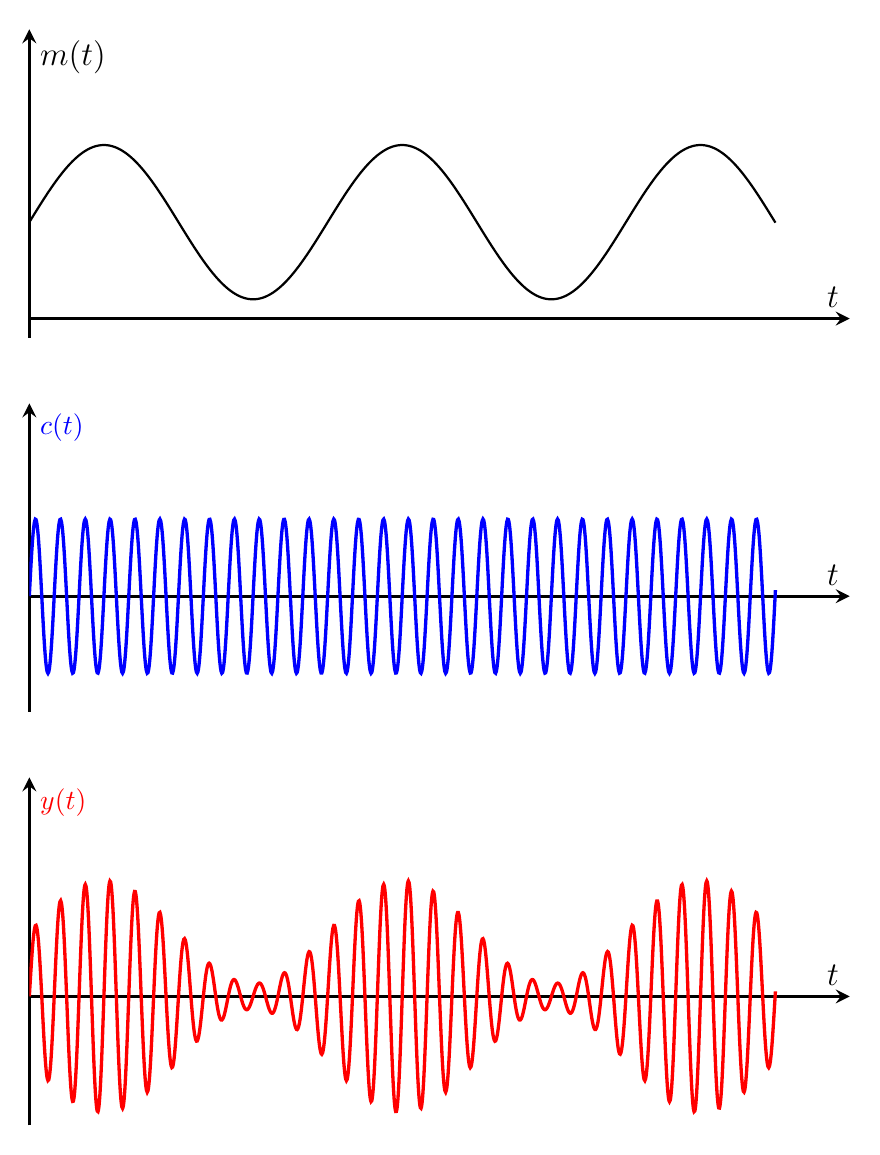
\begin{tikzpicture}[samples=1000, domain=0:10*pi]
				
				\begin{axis}[
				width=12cm, height=5.5cm,
				xtick=\empty,
				ytick=\empty,
				xlabel={\large $t$},
				ylabel={\large $m(t)$},
				xmin=0, xmax=11*pi,
				ymin=-0.5, ymax=7.5,
				axis lines = middle,
				very thick,
				trig format = rad
				]
				\addplot [no markers, smooth, thick] {2.5 + 2*sin(0.5*x)};
				\end{axis}
				
				\begin{axis}[
				at={(0, -4.75cm)},
				width=12cm, height=5.5cm,
				xtick=\empty,
				ytick=\empty,
				xlabel={\large $t$},
				ylabel={\textcolor{blue}{$c(t)$}},
				xmin=0, xmax=11*pi,
				ymin=-3, ymax=5,
				axis lines = middle,
				very thick,
				trig format = rad
				]
				\addplot [no markers, smooth, blue, very thick] {2*sin(6*x)};
				\end{axis}
				
				\begin{axis}[
				at={(0, -10cm)},
				width=12cm, height=6cm,
				xtick=\empty,
				ytick=\empty,
				xlabel={\large $t$},
				ylabel={\textcolor{red}{$y(t)$}},
				xmin=0, xmax=11*pi,
				ymin=-10, ymax=17,
				axis lines = middle,
				very thick,
				trig format = rad
				]
				\addplot [no markers, smooth, red, very thick] {(2.5 + 2*sin(0.5*x)) * 2*sin(6*x)};
				\end{axis}
				\end{tikzpicture}
			\end{center}
			\begin{center}
				The signal in red \textit{i.e.,} $y(t)$ is the \textit{amplitude modulated} wave.
			\end{center}
		Generally we have the modulated signal as $y(t)=m(t).c(t)$, but in case of amplitude modulation if we use this form, there is a serious problem of phase reversal \textit{i.e.,} the signal crosses the $x-axis$, which in turn when multiplication causes the problem of phase reversals.
		\end{flushleft}
		\begin{center}
			\includegraphics[width=0.60 \textwidth]{./SDC-Phase Reversal_1.png}
		\end{center}
		The mechanism of retrieval of original message signal from such a phase reversed signal is complicated and impractical for implementation. So, we improvise and solve this problem.\\\smallskip
		To do so, we shift our message signal $m(t)$, by some \textit{DC} value say $A$ and then multiply it with its carrier signal, for modulation purposes.\\\smallskip
		The general form of such signal is given by the following equation,
		\begin{equation}
			y(t)=A_c [1+k_a m(t)]cos(2 \pi f_c t)
		\end{equation}
		From the above equation if we observe then, the message signal is measured in $volts$. Therefore, by dimensional analysis the unit of $k_a$ is $volts^{-1}$.So,\\\smallskip
		$k_a$, is the amplitude sensitivity.\\
		$m(t)$ is the message/modulating signal.\\
		$y(t)$ is the modulated wave.\\\smallskip
		The \textit{envelope} of $y(t)$ in particular has same shape as the baseband signal $m(t)$ provided that the following two requirements are satisfied,
		\begin{itemize}
			\item{
				The amplitude of $k_a m(t)$ represented as $|k_a m(t)|$ is always less than unity,\textit{i.e.,}
				\begin{equation}
					|k_a m(t)| \leq 1,\enspace \forall \enspace t
				\end{equation}
				\begin{itemize}
					\item{It ensures that the function $1+k_a m(t)>0$, and since an envelope is positive. We can represent it as $A_c [1+k_a m(t)]$.}
					\item{When, $|k_a m(t)|>1$, $y(t)$ becomes overmodulated, resulting in carrier phase reversals whenever the factor as mentioned $1+k_a m(t)$ crosses zero.
					\item{The absolute maximum value of $k_a m(t)$ multiplied by $100$ is referred to as \textit{percentage modulation}}}
				\end{itemize}
			}
			\item{
				The carrier frequency $f_c$ is much greater than the highest frequency component $W$ of the message signal $m(t)$\textit{i.e.,}
				\begin{equation}
					f_c \gg W
				\end{equation}
				\begin{itemize}
					\item{If the above condition is not satisfied, an envelope cannot be realized successfully. The component $W$, is called the message bandwidth.}
				\end{itemize}
			}
		\end{itemize}
		
		If we take the \textit{fourier} transform of \textit{equation} (), then we have,
		
		\begin{center}
		$$F(y(t))=Y(f)=\int_{-\infty}^{\infty} A_c [1+k_a m(t)]cos(2 \pi f_c t) dt$$\\\smallskip
			\begin{flushleft}
				Upon, using the following results we simplify the above equation,\\\smallskip
			\end{flushleft}
			\begin{itemize}
				\item{$cos(x)=\dfrac{e^x-e^{-x}}{2}$}
				\item{$\int_{-\infty}^{\infty} e^{j 2 \pi f (t-a)} df=\delta (t-a)=\delta (a-t)$}
			\end{itemize}
			
		\end{center}
		We find that,
		\begin{equation}
			F(cos(2 \pi f_c t))=\dfrac{\delta(f-f_c)+\delta(f+f_c)}{2}
		\end{equation}
		\textit{equation} $Y(f)$ implies,
		\begin{equation}
		Y(f)=\dfrac{A_c}{2}[\delta(f+f_c)+\delta(f-f_c)]+\dfrac{k_a A_c}{2}[M(f+f_c)+M(f-f_c)]
		\end{equation}
		\subsection{Types of Amplitude Modulation}
		\begin{flushleft}
			\begin{itemize}
				\item{\textbf{Double Side Band - with Carrier(DSB-WC)} : This form of Amplitude Modulation is most widely used. All radio channels in the AM band use this type of modulation.}
				\item{\textbf{Double Side Band - Suppressed Carrier(DSB-SC)} : This form of Amplitude Modulation is same as the above mentioned except for the fact that it is without carrier(\textit{suppressed}).}
				\item{\textbf{Single Side Band (SSB)} : In this form of AM the only half of the signal of DSB-SC is used.}
				\item{\textbf{Vestigial Side Band (VSB)} : This is the modified version of SSB, to ease the generation and reception of the signal.}
			\end{itemize}
		\end{flushleft}
		\subsection{Advantages}
		\begin{flushleft}
			conten
		\end{flushleft}
	\end{flushleft}
	\pagebreak
	\section{Frequency Modulation}
	\pagebreak
	\section{Experimentation}
	\pagebreak
	\section{Simulation}
	\pagebreak
	\section{Code}
	\pagebreak
	\section{Attenuation}
	\pagebreak
	\section{Demodulation}
	\pagebreak
 	
\end{document}